%\documentclass[journal,10pt,onecolumn,draftcls]{IEEEtran}
\documentclass[journal,10pt,onecolumn]{IEEEtran}
\usepackage{listings}
\usepackage{wrapfig}
\usepackage{graphicx}
\usepackage{float}
% correct bad hyphenation here
\hyphenation{op-tical net-works semi-conduc-tor}


\begin{document}
%
\title{Individual Project 1: OpenMP}
%

\author{Jeremy Wright}

% The paper headers
\markboth{CSE430 Individual Project 1: OpenMP}
{CSE430 Individual Project 1: OpenMP}

% make the title area
\maketitle


\begin{abstract}
%\boldmath
Parallel code is difficult to write and test, however the OpenMP's set of 
extensions allow one to add coarse grained parallelism to a system. This paper 
is a look transforming a formerly serial program into a highly parallel one using 
only OpenMP constructs.
\end{abstract}

\listoffigures
%\newpage 

\IEEEpeerreviewmaketitle

\section{Introduction}

\IEEEPARstart{O}{penMP} allows one to quickly sprinkle bits of parallelism throughout
a serial program and using a profiler such as Intel's Parallel Studio Amplifier, measure 
the speedup.  OpenMP, however, is not a panacea for all parallelism. For example, OpenMP primitives
cannot parallelize C++ iterators.  Despite these 
subtle limitations, OpenMP is an extremely powerful platform for introducing parallelism
into applications and algorithms.  We use Conway's game of life as a conduit to how 
data decomposition is an important component in accelerating parallel programs. Then we 
use intentionally unbalanced matrices to demonstrate OpenMP's loading mechanisms.

\hfill \today

\section{Game of Life}
Conway's Game of Life is a dramatic demonstration that a seemingly complex system,
such as cell mitosis can be governed by a set of simple rules. As a demonstration of
OpenMP's simplicity I implemented a single class drive the Game of Life. Then by 
overriding a few key methods, dynamically run different threading models. 

% needed in second column of first page if using \IEEEpubid
%\IEEEpubidadjcol
\subsection{Data Decomposition}
I defined three threading models, each with a unique decomposition, to test OpenMP's performance impact.
I use 3 segmentations: division by rows, division by columns, 
division by regions.  The Intel Parallel Studio Tools were key to measuring impact of OMP
for each decomposition. 

\begin{figure*}[!h]
\begin{center}
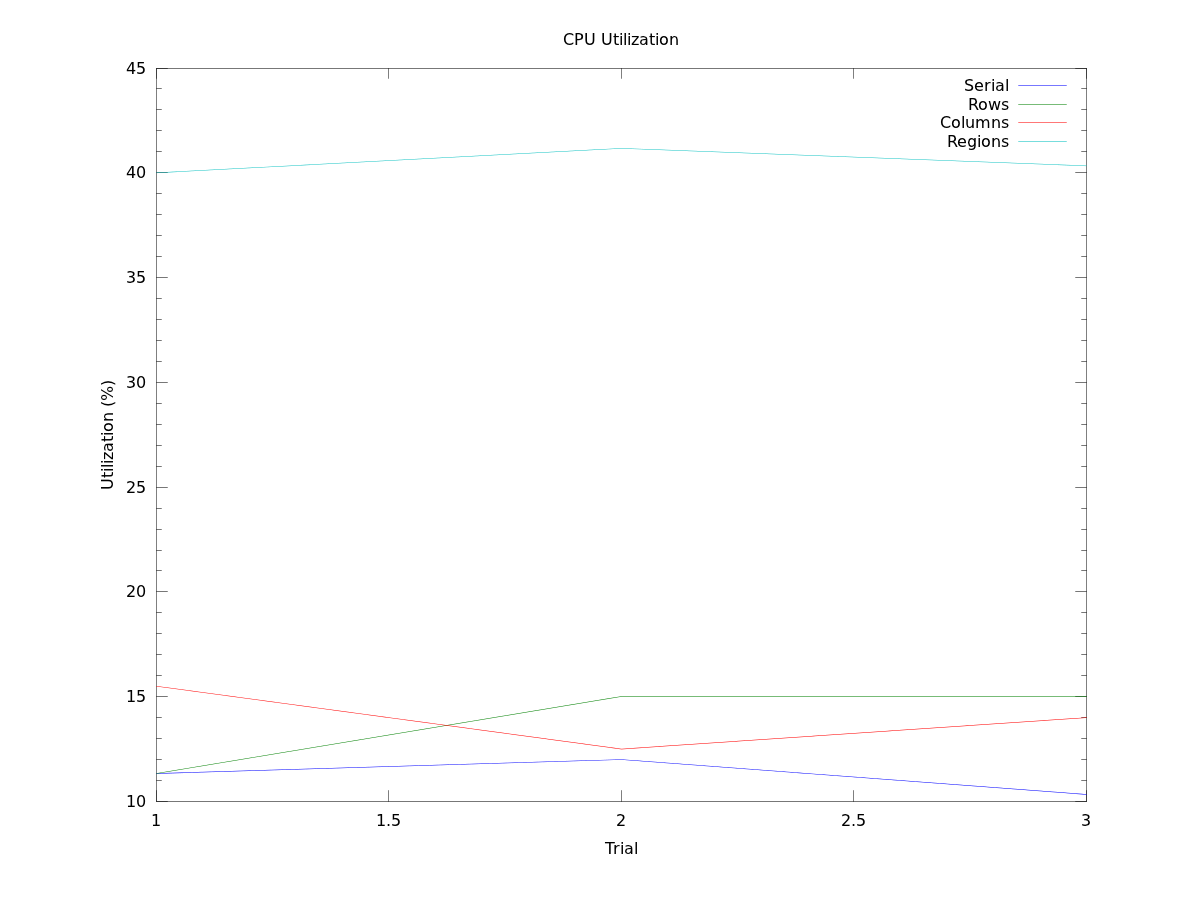
\includegraphics[width=0.8\textwidth]{figures/utilization_compared.png}
\caption{CPU Utilization between different threading models on a 6 core machine.}
\label{fig:gol_cpu_utilization}
\end{center}
\end{figure*}

All tests were run on a 6-core AMD Phenom II processor, in Linux. Figure~\ref{fig:gol_cpu_utilization},
is a dramatic illustration of the performance boost OMP offers.  The row and column divisions are not 
surprisingly similar, however I was surprise to find that the performance of either was not much better 
than the single threaded model.  Decomposing the Game of Life into regions offered a dramatic
boost is CPU utilization.

Each successive threading model simply uses more parallel-for constructs.  Its surprisingly easy
to add parallelism to a serial application using OpenMP.  See section~\ref{sec:Intel-Tools} for how the 
Intel Parallel Studio tools help to find data races, and further analyse threading performance.

\section{Matrix Multiplication}

\subsection{Intertask Dependency}
Spawning a thread has some fixed cost, an overhead.  Ergo, it is important that the thread has some 
useful work to do, furthermore a set of threads should be reasonably balanced so the threads will 
finish at about the same time.  First, I chose to directly calculate a balance between the threads,
until I found the dynamic scheduler in OpenMP offers a simpler, yet higher performance result.

\subsubsection{Manual Load Balance}

The task here is to multiple a matrix against an upper triangular matrix.  Equation~\ref{eq:recursive_form}
describes the number of non-zero terms in a range of columns where a and b define column numbers.  
\begin{equation}
\sum\limits_{a}^b (i + 1) = \frac{-(a + b + 2)(a - b -1)}{2}
\label{eq:recursive_form}
\end{equation}
Using this equation one can balance the number of 
multiplications across sets of columns.  To balance the load of a 2000 column matrix 
across 6 processors we have equations~\ref{eq:expanded_form_start} through \ref{eq:expanded_form}.
\begin{eqnarray}
\label{eq:expanded_form_start}
\lefteqn{\frac{-(0 + b + 2)(0 - b -1)}{2}} \\
& = & \frac{-(b + c + 2)(b - c -1)}{2} \\
& = & \frac{-(c + d + 2)(c - d -1)}{2} \\
& = & \frac{-(d + e + 2)(d - e -1)}{2} \\
& = & \frac{-(e + 1999 + 2)(e - 1999 -1)}{2}
\label{eq:expanded_form}
\end{eqnarray}

\begin{figure*}[!t]
\begin{center}
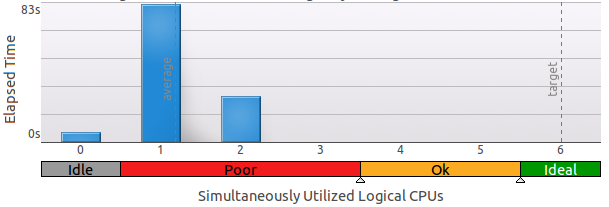
\includegraphics[width=0.8\textwidth]{figures/matrix_without_dynamic_schedule_cpu_usage.png}
\caption{Matrix Multiply Poor CPU Utilization using Standard Parallel for.}
\label{fig:matrix_wo_dynamic_schedule_cpu_usage}
\end{center}
\end{figure*}

\begin{figure*}[!t]
\begin{center}
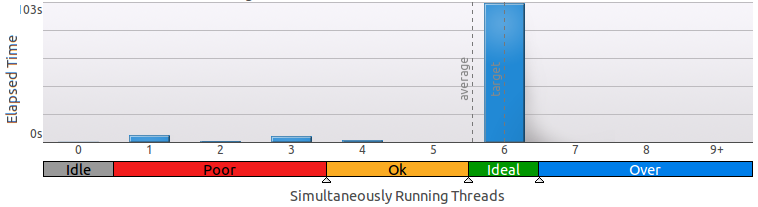
\includegraphics[width=0.9\textwidth]{figures/matrix_without_dynamic_schedule_thread_concurrency.png}
\caption{Matrix Multiply Thread Concurrency using Standard Parallel for.}
\label{fig:matrix_wo_dynamic_schedule_concurrency}
\end{center}
\end{figure*}
Using Newton's method one can find a solution. This will determine the precise slice of
 columns which will give an even work load. 
Despite the precision of this solution the time to compute and the additional bookkeeping
is difficult to justify. Applying this method results in a poor load balance.  
Figure~\ref{fig:matrix_wo_dynamic_schedule_concurrency} demonstrates that the threads have a high 
concurrency, but, as Figure~\ref{fig:matrix_wo_dynamic_schedule_cpu_usage} shows, a very poor CPU 
utilization. This shows that the bookkeeping has a diminishing 
return and luckily OpenMP offers a simpler, automatic solution.

\subsection{Dynamic Load Balance}
OpenMP offers a number of optional parameters called clauses. The scheduling clause allows
for a dynamic load balancing across the OpenMP threads.  

\lstset{language=C,
    breaklines=true,
    basicstyle=\footnotesize,
    caption={Automatic Load Balancing with schedule clause},
    captionpos=b}
\label{lst:AutomaticLoadBalancing}
\begin{lstlisting}
int const chunk = size%omp_get_num_threads();
#pragma omp parallel for schedule(dynamic, chunk)
\end{lstlisting}
Solving this load imbalance is simple as code Listing 1 shows.
The Intel Amplifier shows that the average performance is nearly centered in the Ideal
section. Both CPU Usage (Figure~\ref{fig:matrix_dynamic_schedule_cpu_usage}) and 
Thread Concurrency (Figure~\ref{fig:matrix_dynamic_schedule_concurrency}) centered in the 
Ideal region. This shows that the dynamic scheduler evenly divides the work across threads, 
while simultaneously keeps the threads well loaded.  No single thread of execution is idling 
excessively.

\begin{figure*}[!t]
\begin{center}
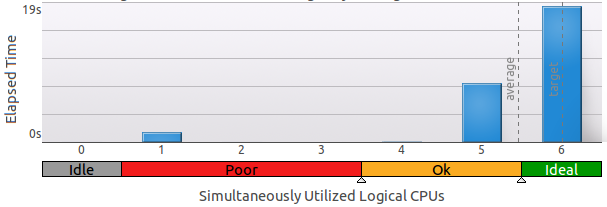
\includegraphics[width=0.8\textwidth]{figures/matrix_dynamic_schedule_cpu_usage.png}
\caption{Matrix Multiply CPU Usage using Dynamic Thread Balancing.}
\label{fig:matrix_dynamic_schedule_cpu_usage}
\end{center}
\end{figure*}

\begin{figure*}[!t]
\begin{center}
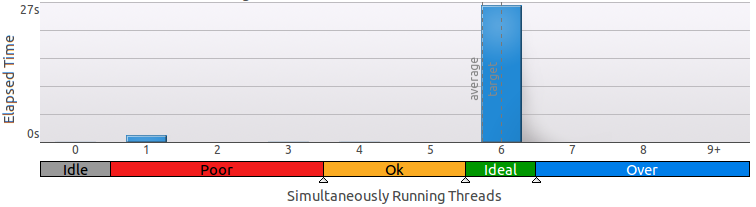
\includegraphics[width=0.8\textwidth]{figures/matrix_dynamic_schedule_thread_concurrency.png}
\caption{Matrix Multiply Thread Concurrency using Dynamic Thread Balancing.}
\label{fig:matrix_dynamic_schedule_concurrency}
\end{center}
\end{figure*}


As more of a curiosity, I wanted to see what more threads would do.  I forced 12 threads 
(Number of Processors * 2).  As Figure~\ref{fig:12_threaded_matrix_cpu_usage} and 
Figure~\ref{fig:12_threaded_matrix_concurrent} show, while the thread concurrency remains
high, the processor is mostly idle.  This is comforting to realize that the OpenMP's default 
settings offer the best performance. This makes using OpenMP in real world project even simpler.


\begin{figure*}[!t]
\begin{center}
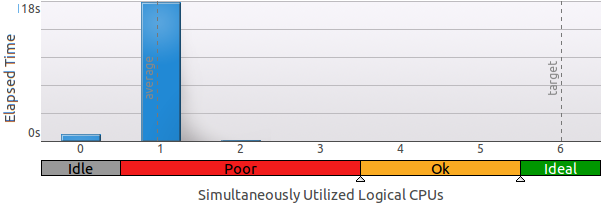
\includegraphics[width=0.8\textwidth]{figures/12_threaded_matrix_thread_cpu_usage_histogram.png}
\caption{CPU Utilization forcing 12 threads.}
\label{fig:12_threaded_matrix_cpu_usage}
\end{center}
\end{figure*}

\begin{figure*}[!t]
\begin{center}
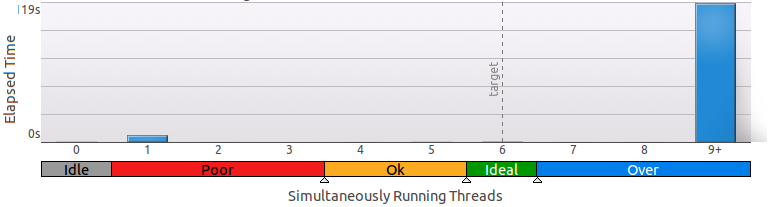
\includegraphics[width=0.8\textwidth]{figures/12_threaded_matrix_thread_concurrent_histogram.png}
\caption{Thread Concurrency forcing 12 threads.}
\label{fig:12_threaded_matrix_concurrent}
\end{center}
\end{figure*}


\section{Conclusion}
OpenMP makes adding parallelism to a given program easy. The constructs allow one to sprinkle
parallel code throughout the program, and the measure the performance boost. Sometimes it
may be prudent to dive in deeper and manually thread some section of code, especially when using
complex C++ constructs such as iterators, but if OpenMP
meets the need, then its a low-cost, cross-platform mechanism.

Furthermore, OpenMP is exposed as a set of \#pragma functions. Since \#pragmas are by 
definition an extension to the language, if the compiler doesn't understand the directives they
are simply ignored. This allows one to liberally use OpenMP, and if the compiler of choice doesn't
support the OpenMP directives, OpenMP will not break the build.  OpenMP is a fantastic tool.

\appendices
\section{Intel Parallel Studio}
\label{sec:Intel-Tools}

\begin{figure*}[!t]
\begin{center}
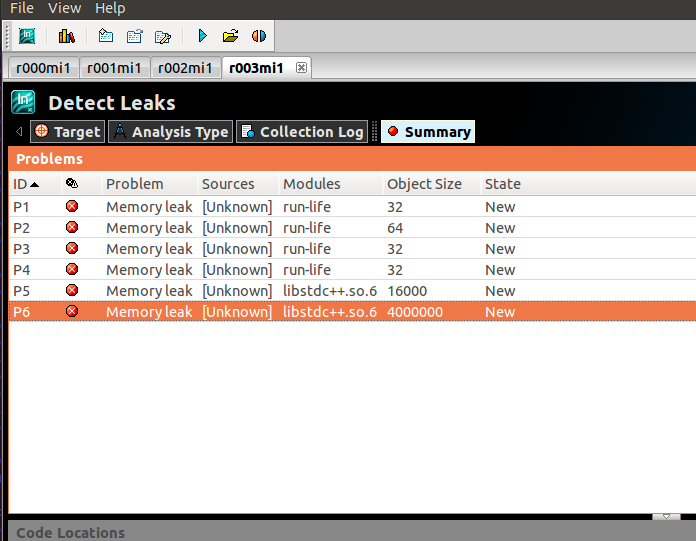
\includegraphics[width=0.8\textwidth]{figures/fileMep7k0_Memory_Analysis.png}
\caption{Intel Inspector with Debug Symbols enabled.}
\label{fig:intentional_memory_leak}
\end{center}
\end{figure*}

\begin{figure*}[!t]
\begin{center}
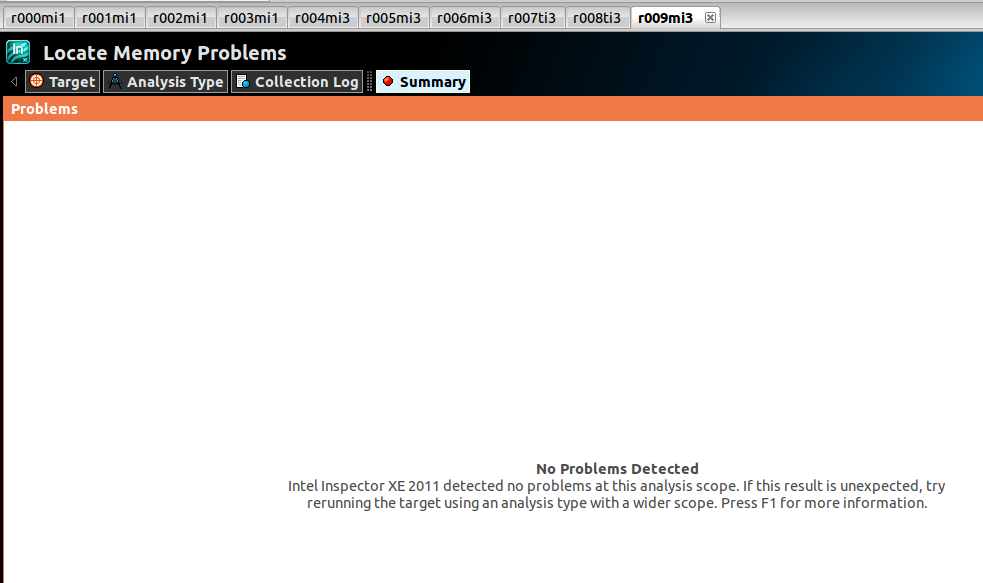
\includegraphics[width=0.5\textwidth]{figures/ChangeSet14_Memory.png}
\caption{Game of Life: All Memory Leaks Fixed.}
\label{fig:inspector_clean_memory}
\end{center}
\end{figure*}

\begin{figure*}[!t]
\begin{center}
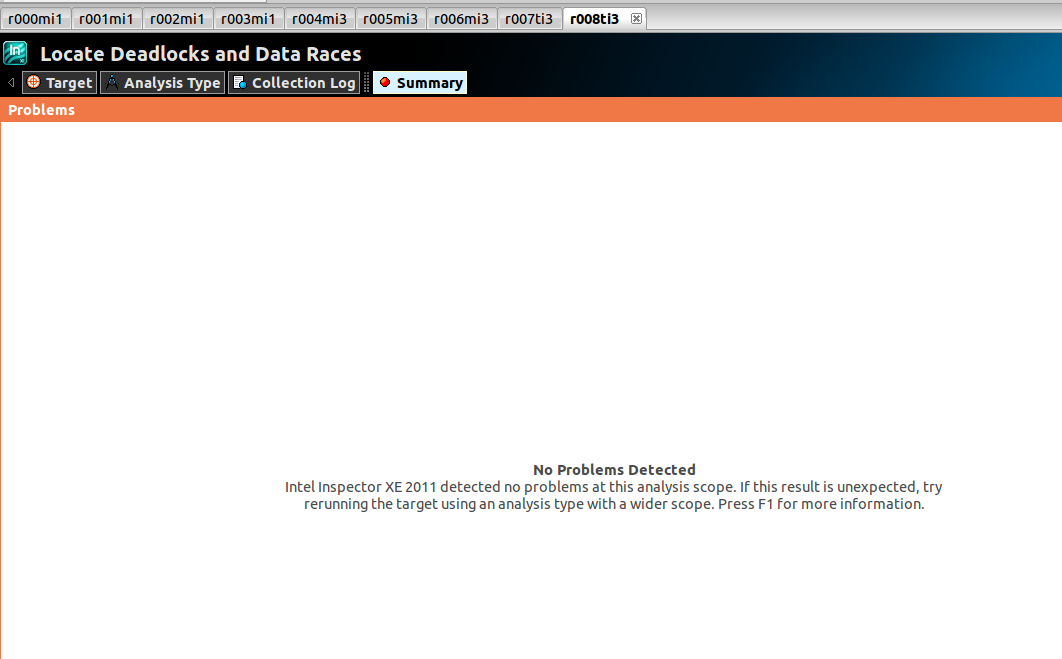
\includegraphics[width=0.8\textwidth]{figures/ChangeSet14.png}
\caption{Game of Life: All Deadlocks and Data Races Fixed.}
\label{fig:inspector_clean_deadlocks}
\end{center}
\end{figure*}

\begin{figure*}[!t]
\begin{center}
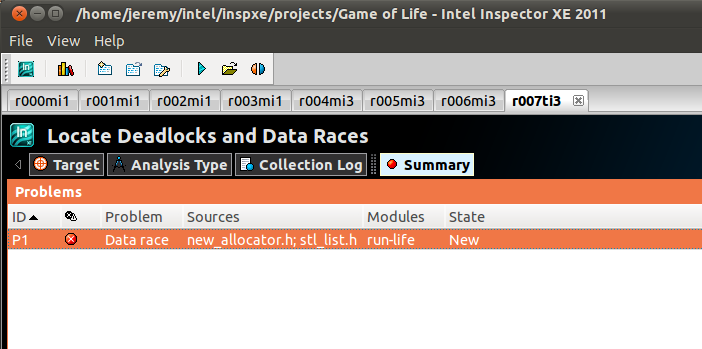
\includegraphics[width=0.8\textwidth]{figures/Data_Race_Anaylsis.png}
\caption{Game of Life: Data Race found on the Update List.}
\label{fig:inspector_data_race_allocator}
\end{center}
\end{figure*}




I was a bit skeptical of the Intel Parallel Studio Tools. I've use Valgrind extensively, and am quite
fond of it. However, I am humbled. Intel Parallel Studio doesn't have the false positive problem
Valgrind does. It is quite satisfying, to see the "No Problem Found" (Figure~\ref{fig:inspector_clean_memory},
Figure~\ref{fig:inspector_clean_deadlocks}).

To evaluate the memory tool, I intentionally omitted a destructor (Figure ~\ref{fig:intentional_memory_leak}).
Intel Parallel Studio doesn't have the learning curve, while you figure out what is innocuous, and which is 
a genuine issue.

For the performance profiling, the profile does slow down execution just as 
Valgrind, but the slowness didn't seem to be as excessive.  The Intel tool 
seemed to profile faster than Valgrind does.  This is purely subjective, as 
I didn't make any comparative measurements.  The only issue I have with the tool suite, is granularity.

The hotspot analysis tool does a great job at identifying heavy-hitter functions and methods. However the
parallel tools need a similar granularity. I acknowledge that some parts of my program are serial; I would 
like a more detailed report to compare the threading performance at given scopes. Ideally, I would
 use \#pragmas to mark scopes with extra analysis, which may be reported separately.

I found the most useful tool was the Data Race analysis (Figure~\ref{fig:inspector_data_race_allocator}).  In
my implementation of game of life I had a shared list that tracked the updates which needed to be committed 
at the end of the generation.  This however caused a data race between multiple threads. I used the OpenMP 
primitives to protect the data, however this destroyed the parallelism (measured with the amplifier). Instead 
I replaced the list with a simple 2D array where each OpenMP thread has it's own copy. Inspector confirms all data
races fixed (Figure~\ref{fig:inspector_clean_deadlocks}), and Amplifier confirms high parallelism.

It's great tool suite. I don't have an Intel processor, so some of the profilers 
wouldn't work, and the errors were non-obvious, but overall the tool is great, and 
I really like that it runs on Linux.



% that's all folks
\end{document}


